\section{Brake Pressure Acquisition Channel}

	A very influential parameter in a braking system is the pressure that the brake exerts on the rotor. Pressure is a magnitude measured in Pascal and can be expressed by the force ratio by the area. There are some sensors based on the piezoelectric effect, but the most accurate way to measure force is by using load cells.

	Load cells have very low output levels, of the level of 2mV/V, and therefore an amplification is fundamental. It is not necessary to know the nature of the strain gauges when a load cell is being calibrated since generally the manufacturers provide a calibration curve based on the signals $V_{O}$ and $V_{EX}$ of the Figure \ref{fig-wheatstone}, it is worth noting that these signals can not have the same reference, otherwise it will not be possible to excite the wheatstone bridge correctly. 

	The most common way to amplify the signal of a load cell is using a instrumentation amplifier. Although it is a widely used configuration, assembling this amplifier using three different operational amplifiers and seven resistors as in Figure \ref{fig-instrumentation-amplifier} may make it inaccurate due to manufacturing imperfections of the components. Another factor that greatly influences the output signal of a load cell is the excitation voltage of its wheatstone bridge, if it varies too much the output will vary greatly as well, which will hamper its calibration.
		
	In order to solve these two problems there is a solution widely used in the market which is the \textit{INA125} of Texas Instruments, this IC besides performing signal amplification also provides a very precise excitation source for the wheatstone bridge, the only component required to be coupled is a resistor $R_{G}$, as shown in Figure \ref{fig-ina125-schematic}. This resistor will determine the gain for the amplification according to the equations \ref{eqn-ina125-vo} and \ref{eqn-ina125-g}:
	

		\begin{figure}[htbp]
			\centering
				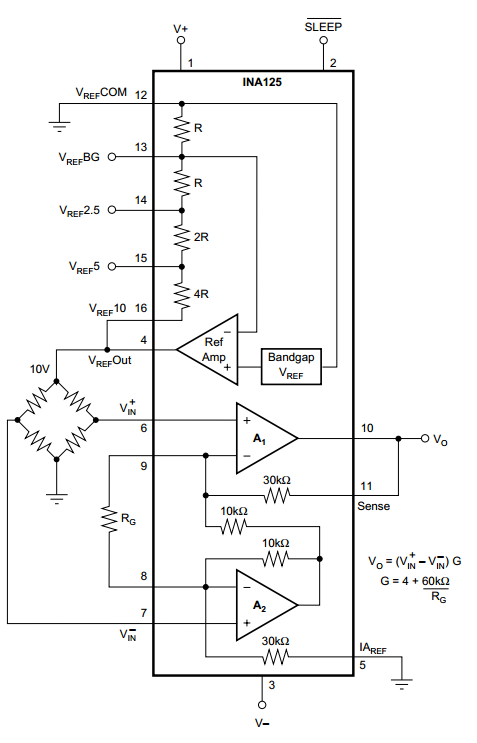
\includegraphics[scale=0.85]{figuras/fig-ina125-schematic.png}
			\caption{INA125 Schematic \cite{ina125data}}
			\label{fig-ina125-schematic}
		\end{figure}

		\begin{equation}\label{eqn-ina125-vo}
			V_{O}=(V_{IN}^{+} - V_{IN}^{-} ) \cdot G
		\end{equation}

		\begin{equation}\label{eqn-ina125-g}
			G=4 + \frac{60k\Omega}{R_{G}}
		\end{equation}

		Taking into account the sensitivity of 2mV/V, this means that if the cell is excited with 10V, its output will vary from 0 to 20mV. Since the analog input of the chosen microcontroller (Atmega328) is 0 to 5V, we may to amplify the cell output signal by a factor of 250 to increase precision. Using Equation \ref{eqn-ina125-g}, to obtain a gain of amplification ratio of the ideal $R_{G}$ would be 243$\Omega$, a resistor of this value is not commercially available, the closest ones would be 240$\Omega$ and 270$\Omega$. The first would cause a gain greater than 250 and consequently an IC output voltage greater than 5V when the cell had an output voltage of 20mV. The resistor 270$\Omega$ will generate a gain of 226 and cause the IC output to range from about 0V to 4.52V, using 90.4\% of the resolution of the microcontroller input. 
		\par

		Figure \ref{fig-cic-cell} shows the schematic of the load cell conditioning circuit with the Texas Instruments INA125 IC.

		\begin{figure}[htbp]
			\centering
				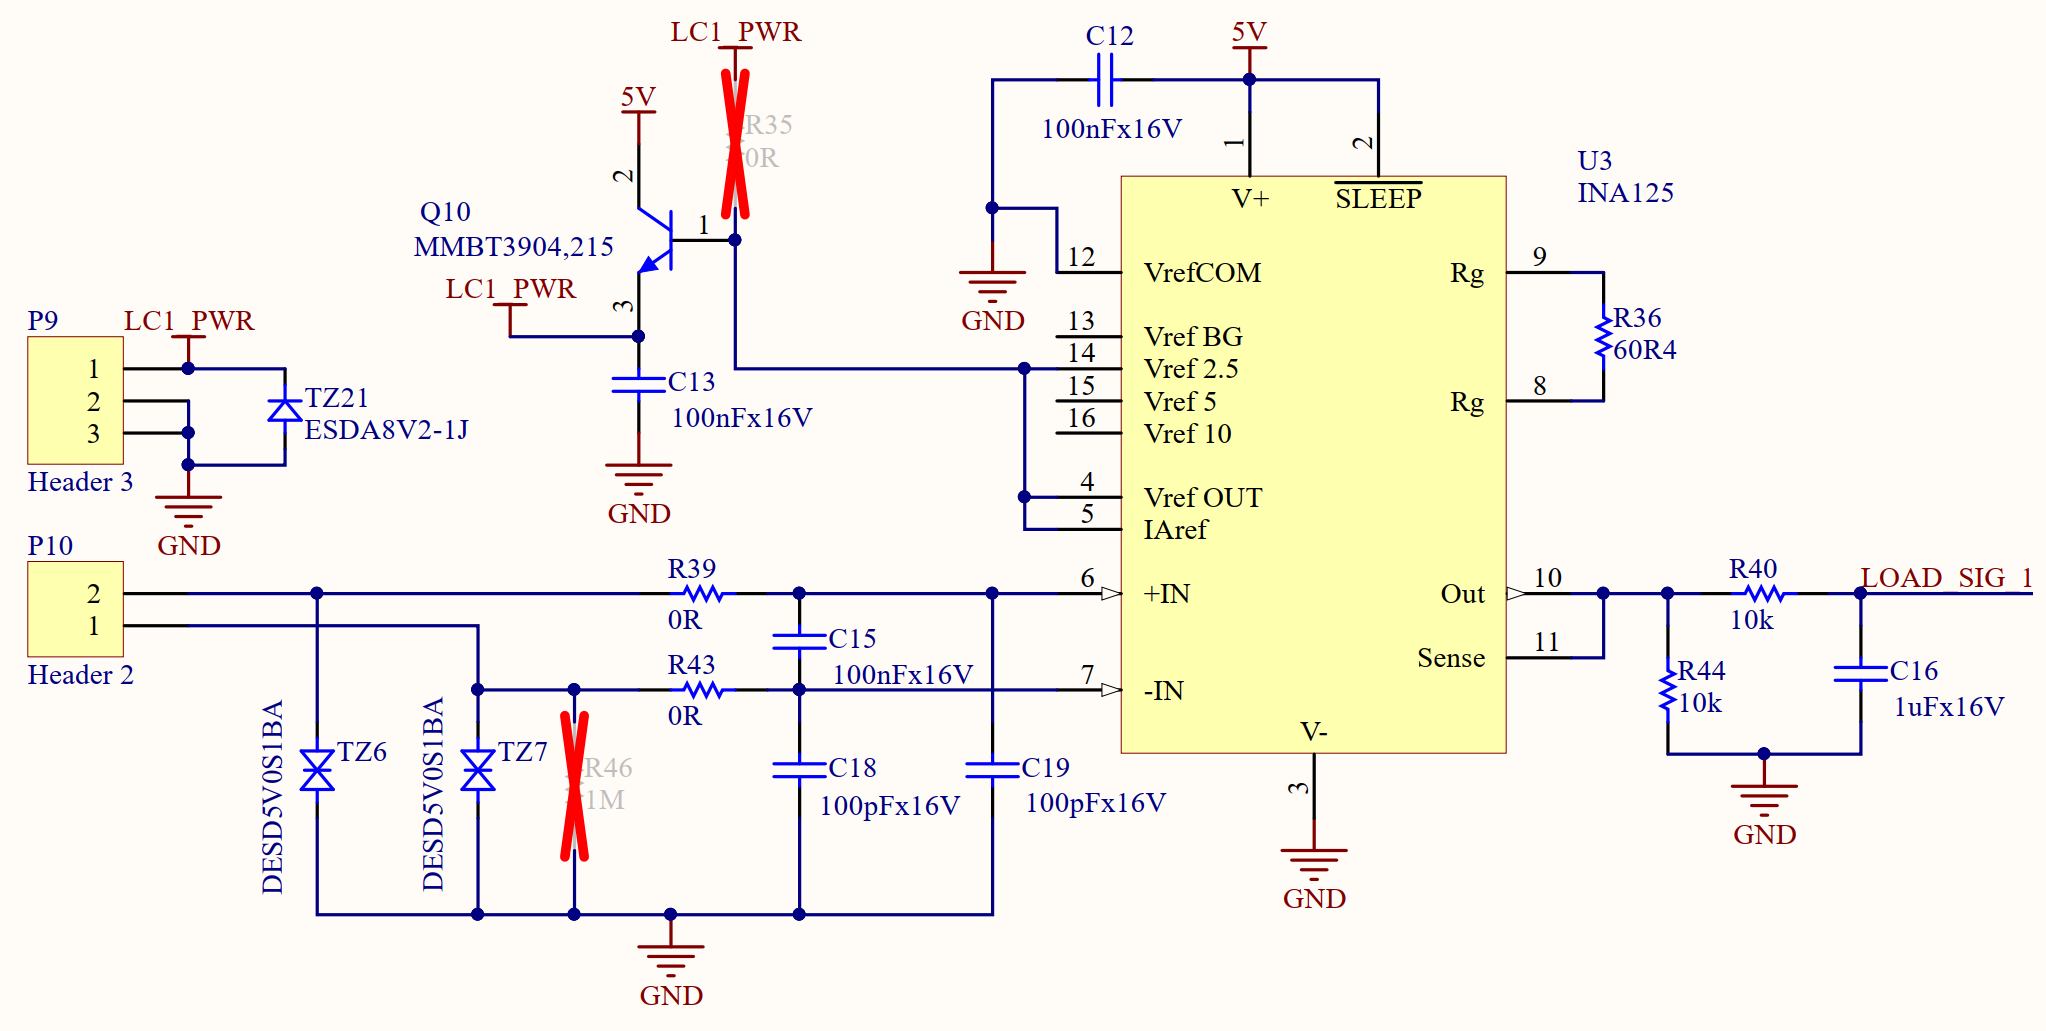
\includegraphics[scale=0.35]{figuras/fig-cic-cell.png}
			\caption{Conditioning Circuit for the Load Cell}
			\label{fig-cic-cell}
		\end{figure}
